%============================================================ 3. 문제 정의 (압축판)
\section{문제 정의와 평가 지표}
\label{sec:problem}

\subsection{교전 시나리오}
\label{sec:scenario}
%============================================================ 교전 시나리오 표 (국방발표 판)
%  저널판은 tables/tab_scenario.tex(자동 생성)를 쓰고 길이를 관측 픽셀 한 변 $\ell$ 단위로
%  적는다. 발표판은 같은 설정을 m·m/s 로 환산해 싣는다 --- 환산 기준은 기준 인스턴스
%  $\ell = 252\unit{m}$, 결정 주기 25\,s 이며, 원값은 학습 체크포인트의 설정이다.
%    교전 해역 한 변 50 \ell = 12.6 km,  적 0.89 \ell/주기 = 9.0 m/s,  방어정 0.60 \ell/주기 = 6.0 m/s
%  ★ 15쪽판은 물리 단위(m·m/s·s)를 싣지 않는다 --- 길이는 관측 픽셀 한 변 ell 단위,
%    속력은 비율만 둔다. 결정 주기·픽셀 크기의 절대값은 위 환산 기준에만 남긴다.
%  표 밑 주석은 싣지 않는다(발표판 방침).
\begin{table}[htbp]
\centering
\caption{교전 시나리오와 관측 설정}
\label{tab:scenario}
\footnotesize
\resizebox{\ifdim\width>\linewidth\linewidth\else\width\fi}{!}{%
\begin{tabular}{lr}
\toprule
항목 & 값 \\
\midrule
적 USV 수 $M$ & 10 \\
방어정 수 $P$ & 3 \\
적 무리 최대 수 $C$ & 4 \\
교전 해역 한 변 & $50\,\ell$ \\
속력비 $v_e/v_a$ (적 USV / 방어정) & 1.5 \\
관측 격자 $n_{\mathrm{g}} \times n_{\mathrm{g}}$ (모선 중심) & $50 \times 50$ \\
방어정당 그물 (학습 / 평가) & 1 / 3 \\
정책 파라미터 수 & 244{,}389 \\
\bottomrule
\end{tabular}
}
\end{table}




교전 해역 중앙에 고가치 모선 한 척이 있고, 가장자리에서 적 USV $M$척이 모선을 향해
돌진한다. 적은 방어정보다 빠르다고 가정하며, 세 공격 포메이션 가운데 하나를
취한다(Fig.~\ref{fig:formations}). 집중(concentrated)은 모든 적이 한 방향에서 몰려오는
형태이고, 양동(diversionary)은 적이 세 방향으로 나뉘어 동시에 접근하는 형태이며,
파상(wave)은 적이 다수의 무리로 나뉘어 같은 방향에서 조금씩 어긋난 경로로 시간차를 두고
차례로 밀려오는 형태이다.

방어정 $P$척은 각각 한정된 수의 그물을 전개할 수 있다. 방어정이 두 경유점 사이를 이동하며
후미의 전개 장치로 부유식 그물을 풀어 놓으면, 그 위를 지나는 적 USV의 추진기관이
무력화된다(Fig.~\ref{fig:netconcept}). 외란에 의한 그물의 위치 변동과 적의 회피 기동을
최대한 줄이기 위해, 방어정은 적이 자신에게 최대한 근접하였을 때 그물을 펼치는 것을 목표로
한다. 세부 설정은 Table~\ref{tab:scenario}에 정리하였으며, 모든 거리는 관측 지도의 한 칸 크기
$\ell$ 을 기준으로 나타내므로 해역의 실제 크기가 달라져도 같은 체계를 그대로 적용할 수 있다.

\begin{figure}[!htbp]
\centering
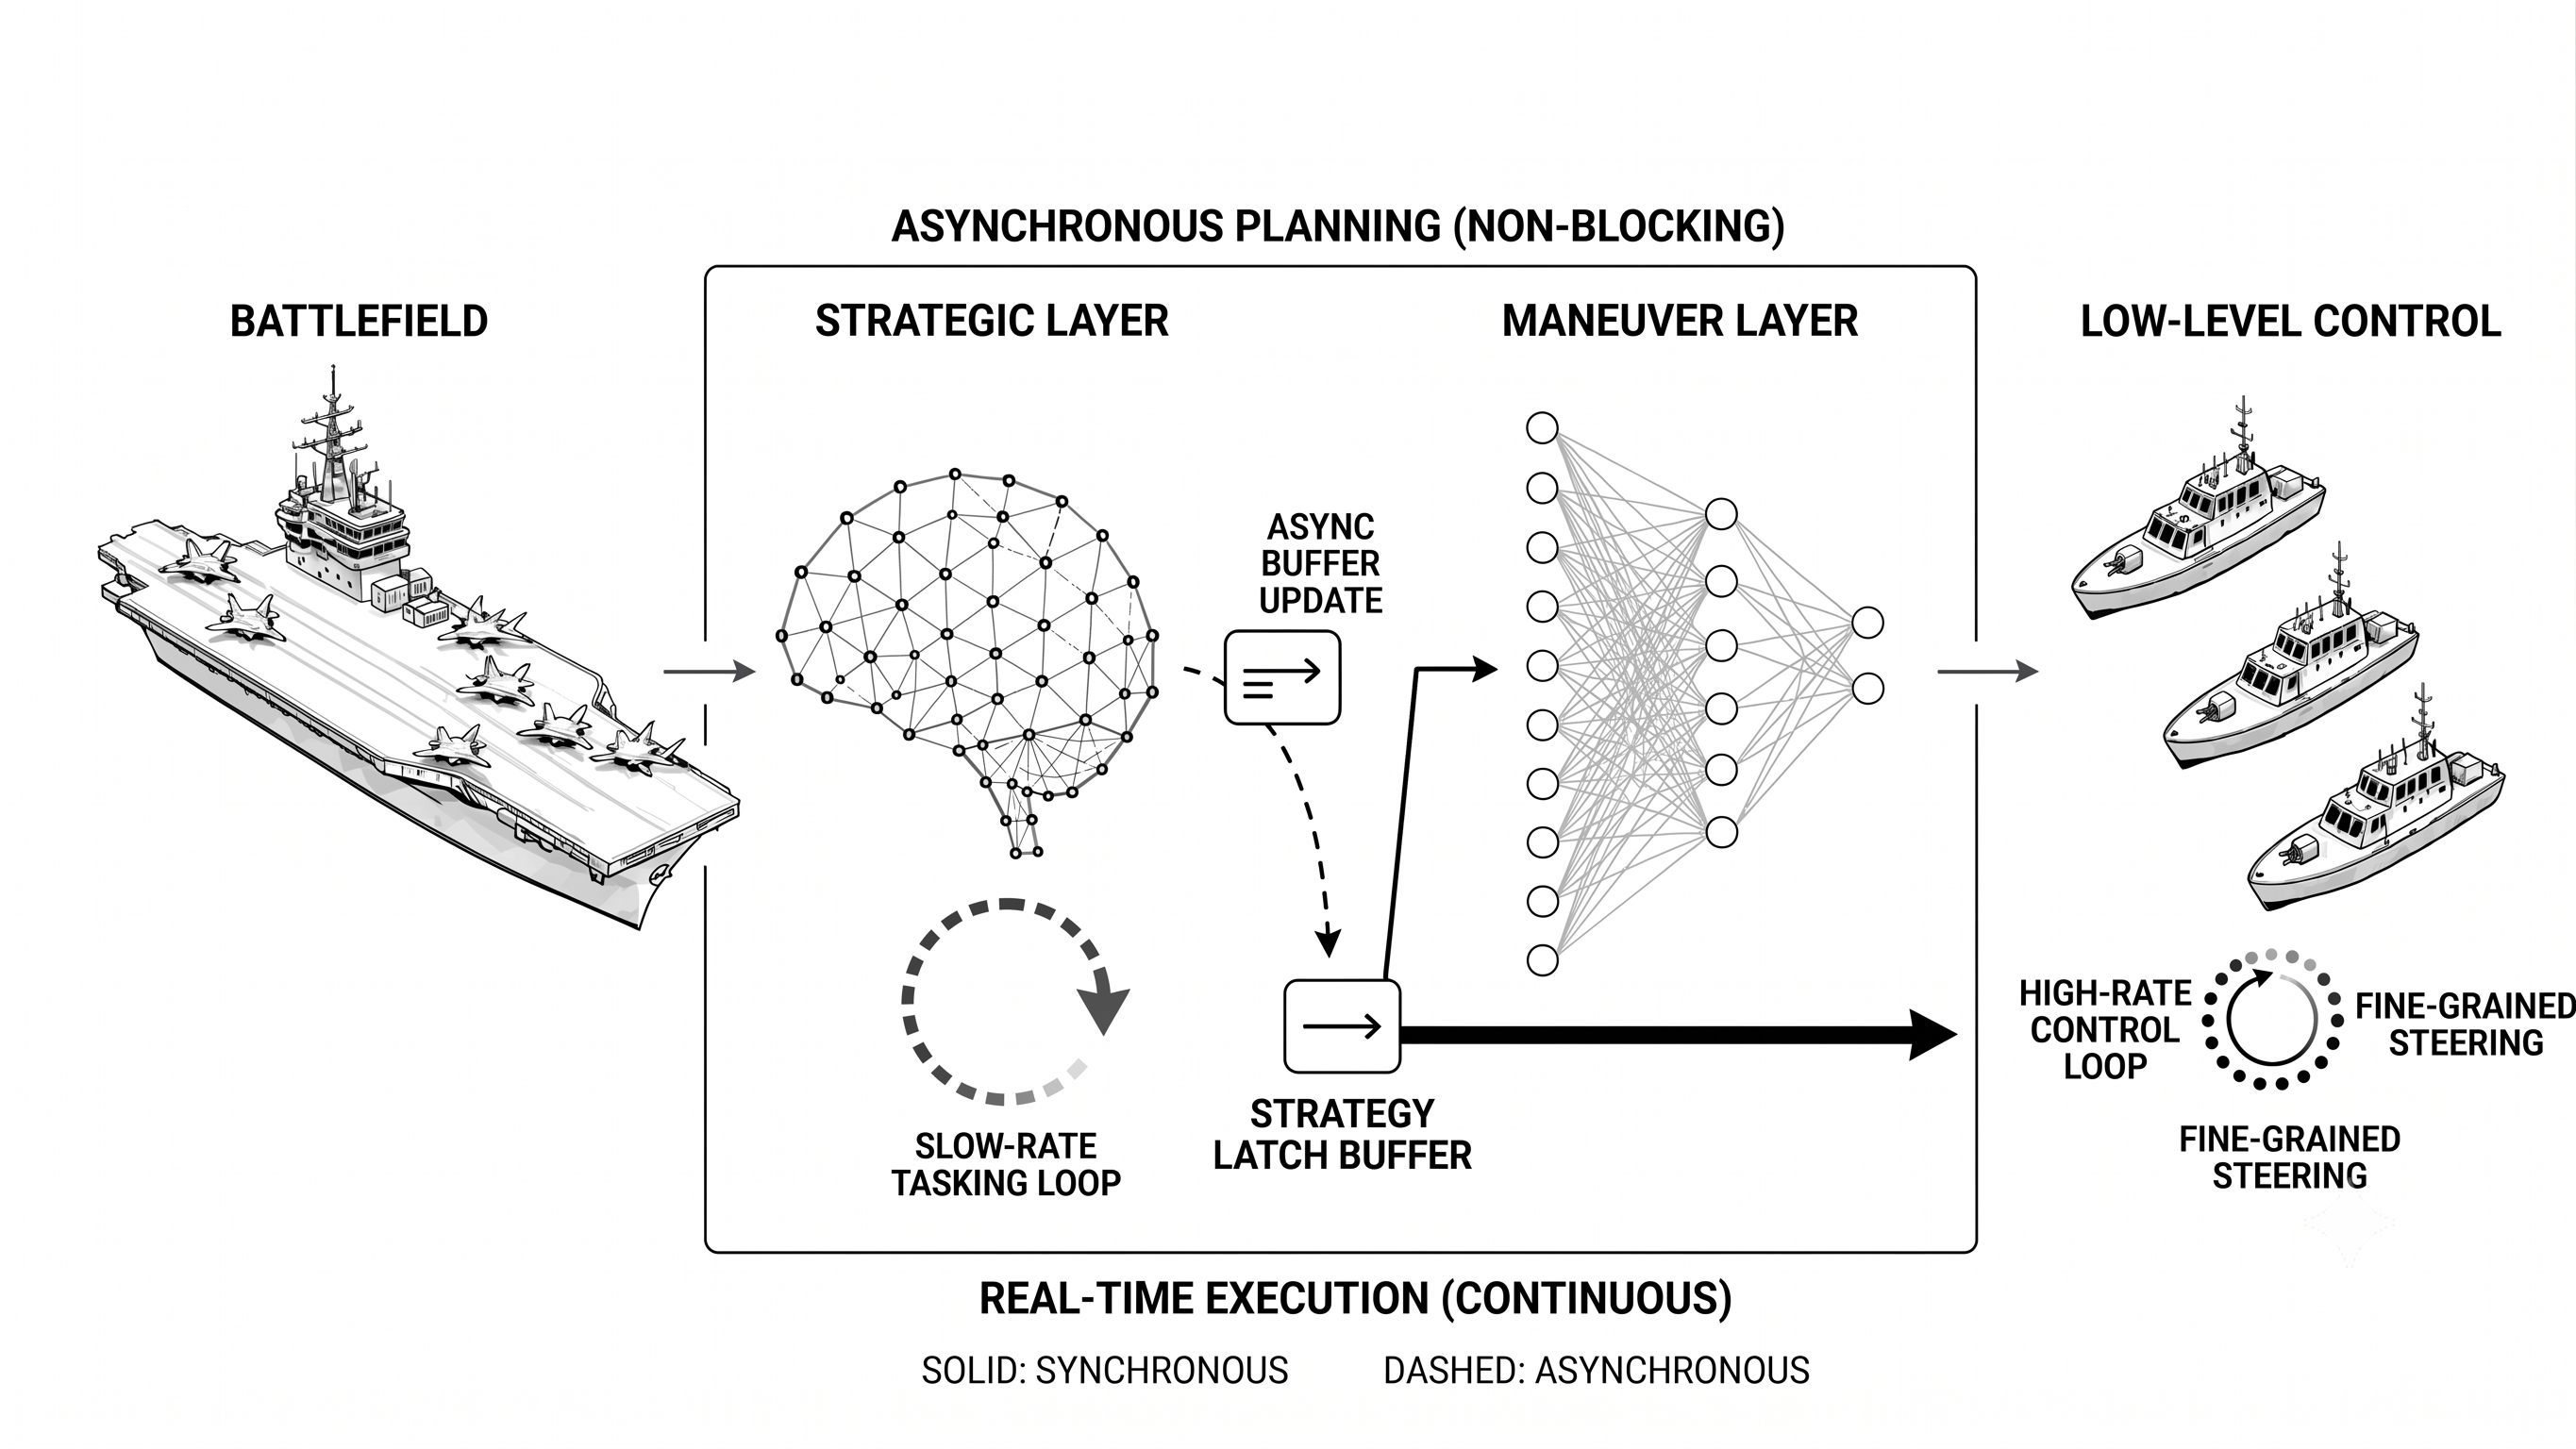
\includegraphics[width=0.62\columnwidth]{fig3.png}
\caption{후미 투하식 부유 그물의 포획 개념}
\label{fig:netconcept}
\end{figure}

\subsection{평가 지표}
\label{sec:metrics}

방어 성과는 다섯 관점의 9개 지표로 에피소드마다 잰다(Table~\ref{tab:metrics}). 모든 에피소드에서
적 USV는 포획되거나 모선에 도달(돌파 수 $N_\mathrm{brc}$)하는 것으로 결판나 돌파 수는 포획률과 같은
정보이므로 따로 두지 않는다. 자원 효율은
교전하지 않은 조건이 가장 효율적으로 보이는 것을 막기 위해 총량이 아니라 포획당 비율로
두었고, 교전 품질은 거리축과 시간축으로 나누어 모선에서 먼 포획과 이른 포획을 함께 본다.

\begin{table*}[!b]
\centering
\caption{평가 지표 9종}
\label{tab:metrics}
\footnotesize
\renewcommand{\arraystretch}{1.25}
\begin{tabular}{llp{0.30\linewidth}p{0.30\linewidth}}
\toprule
관점 & 지표 & 정의 & 뜻 \\
\midrule
방어 성과
 & 포획률           & $\capr = N_\mathrm{cap} / (N_\mathrm{cap} + N_\mathrm{brc})$ & 결판난 적선 중 포획 비율 \\
\midrule
\multirow{2}{*}{안전}
 & 충돌률           & $N_\mathrm{col} / P$ & 방어정당 아군·모선 충돌 \\
 & 그물 걸림        & $N_\mathrm{tng}$ & 아군 그물에 얽힌 횟수 \\
\midrule
\multirow{2}{*}{자원 효율}
 & 포획당 그물      & $N_\mathrm{net} / N_\mathrm{cap}$ & 포획 1건당 그물 소모 \\
 & 포획당 이동거리  & $\sum_{p=1}^{P} D_p \,/\, N_\mathrm{cap}$ & 포획 1건당 팀 이동거리 \\
\midrule
기동 비용
 & 총 선회량        & $\sum_{p=1}^{P} \sum_{t} \lvert \Delta\psi_{p,t} \rvert$ & 누적 방위 변화(궤적 평활도) \\
\midrule
\multirow{3}{*}{교전 품질}
 & 포획 이격거리    & $\frac{1}{N_\mathrm{cap}} \sum_{k} \lVert \mathbf{z}_k - \mathbf{m} \rVert$ & 포획 지점의 모선 거리 \\
 & 평균 포획 시각   & $\frac{1}{N_\mathrm{cap}} \sum_{k} t_k$ & 포획이 일어난 시각 \\
 & 전개 시 적 거리  & $\frac{1}{N_\mathrm{net}} \sum_{d} \min_{m \in \mathcal{A}} \lVert \mathbf{a}_d - \mathbf{e}_m \rVert$ & 그물 전개 시 최근접 적 거리 \\
\bottomrule
\end{tabular}
\end{table*}
